\chapter{Machine Learning Diagnostic}


\section{Splitting dataset}
\begin{itemize}
    \item To implement a diagonostic test, data sets can be divided into three parts: \textbf{training set} 60\%, \textbf{cross validation set} 20\% and \textbf{test set} 20\%.
    
    \begin{itemize}
        \item \textbf{training set}: to train the different candidate models during the learning process
        \item \textbf{validation set}: to compare performances of these models and decide which one to take, that is to tune the hyperparameters
        \item \textbf{test set}: only to assess the performance such as accuracy, sensitivity, specificity, F-measure, and so on
    \end{itemize}

    \item The cost functions of each sets would be $J_{\text{train}}$, $J_{\text{cv}}$, $J_{\text{test}}$

\end{itemize}


\section{Model selection}
\begin{itemize}
    \item Diagnose degree of polynomial
    \begin{figure}[H]
        \centering
        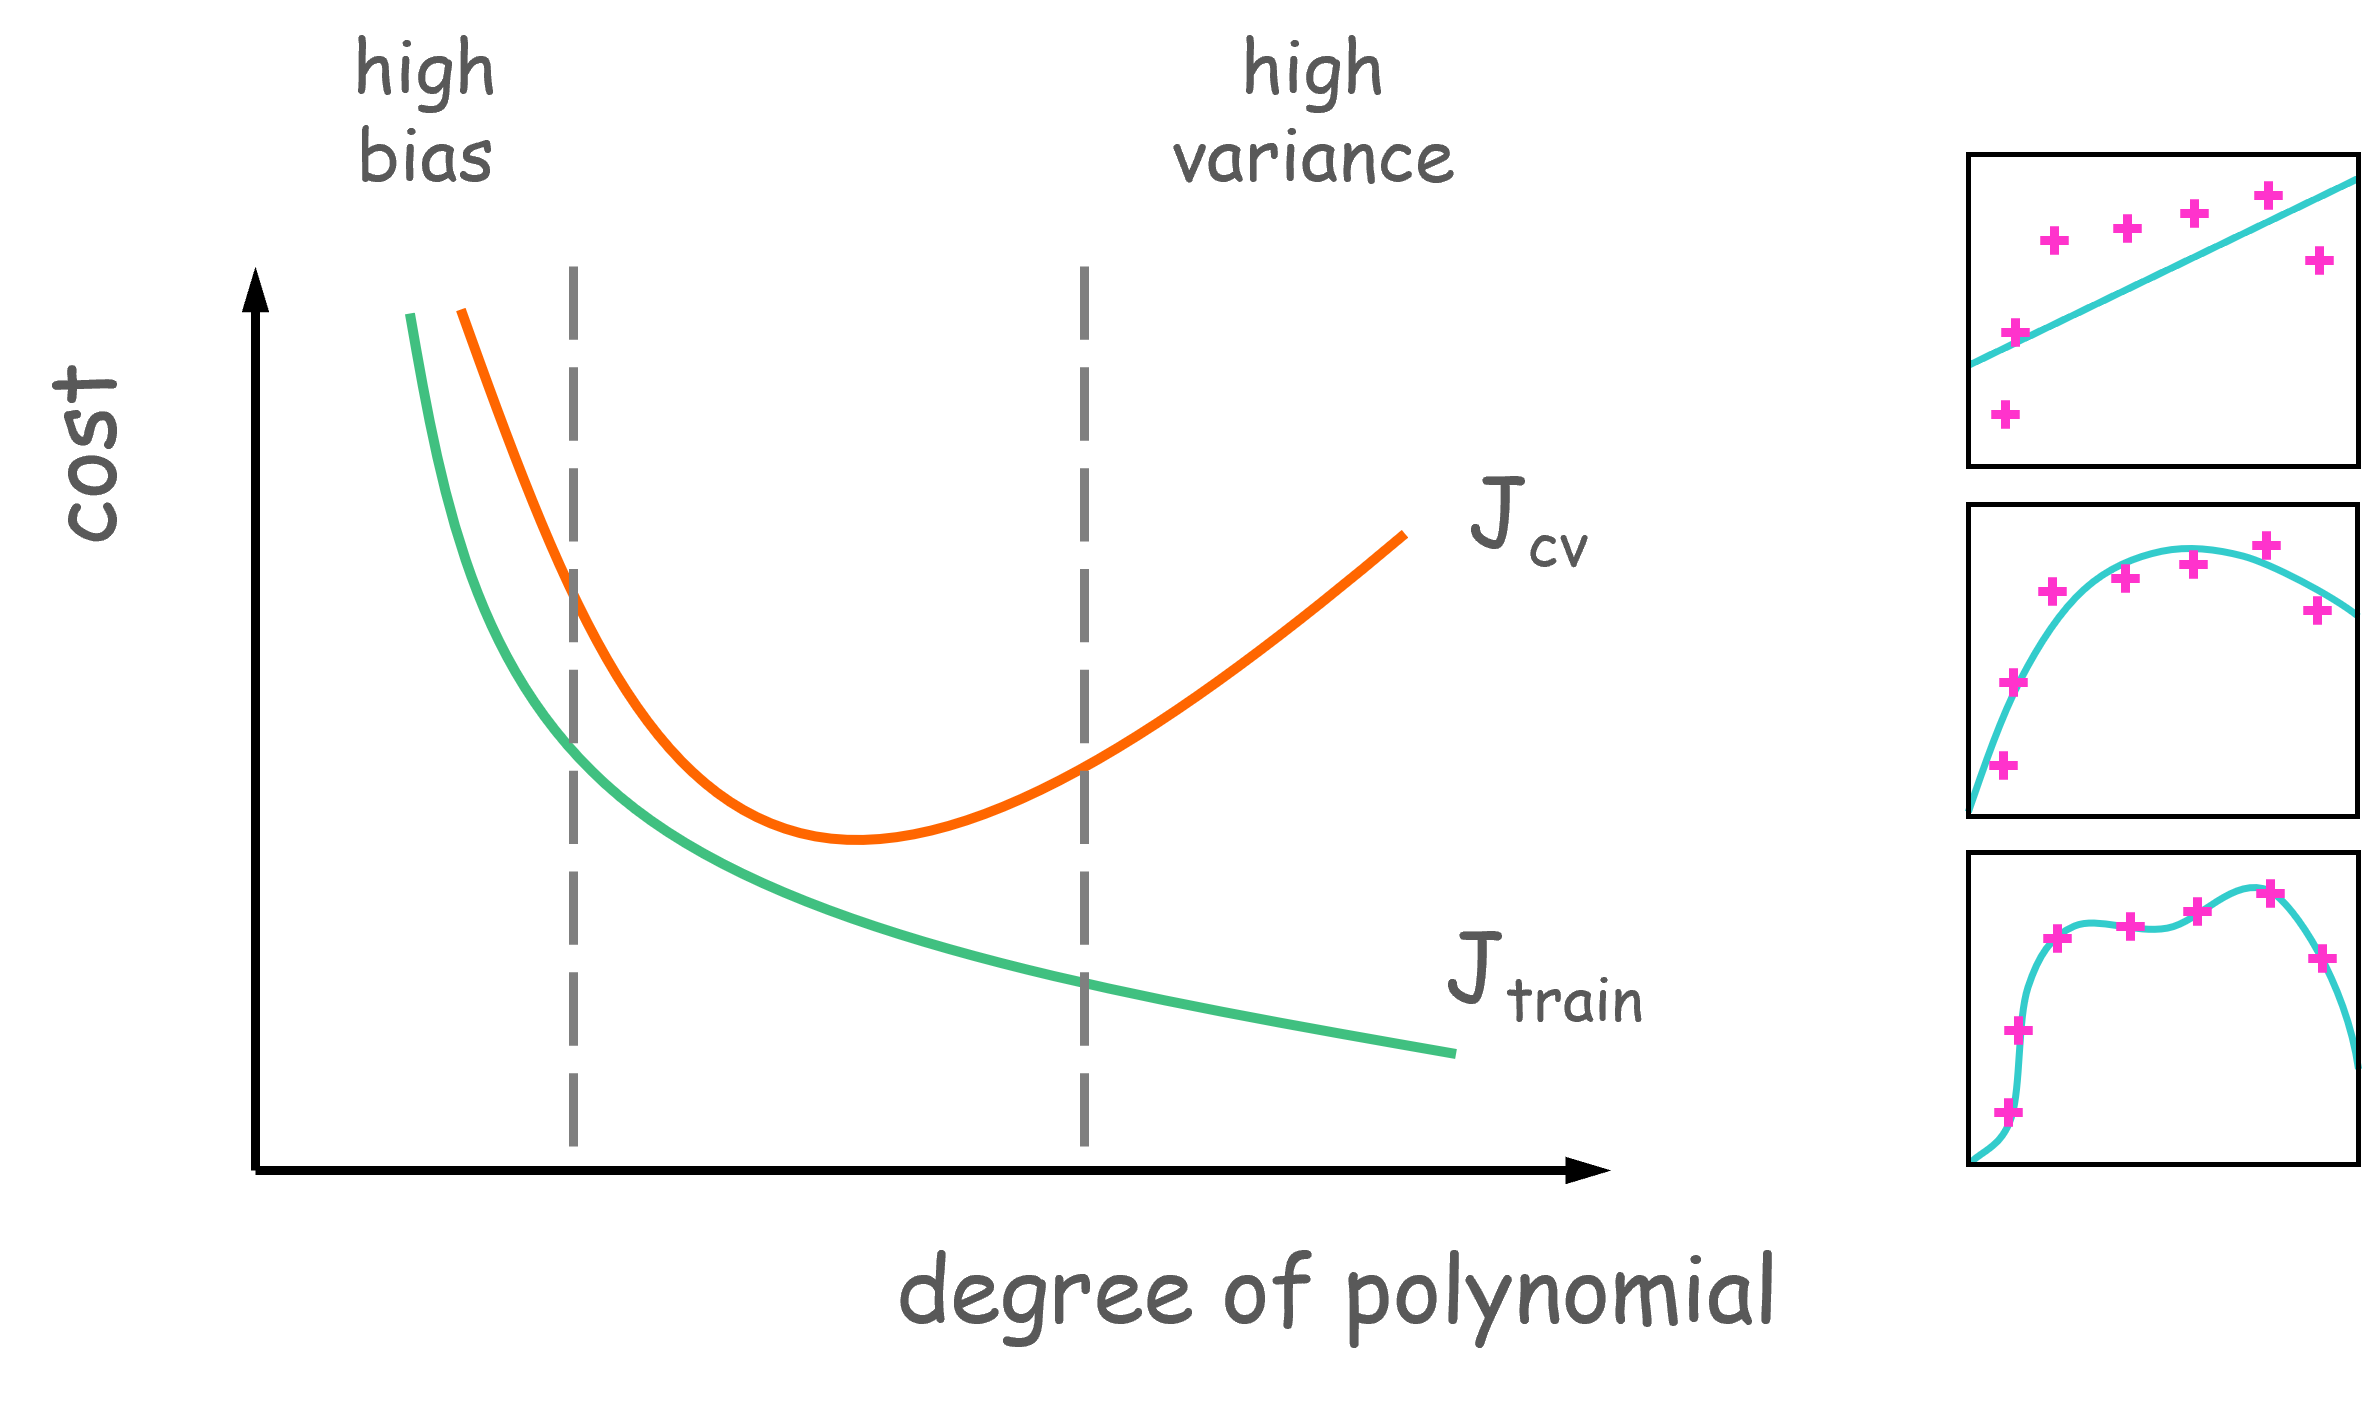
\includegraphics[width=3.8in]{./images/diagnose_degree_of_polynomial.png}
        \caption{Diagnose degree of polynomial $d$}
    \end{figure}

    \item Diagnose regularization parameter
    \begin{figure}[H]
        \centering
        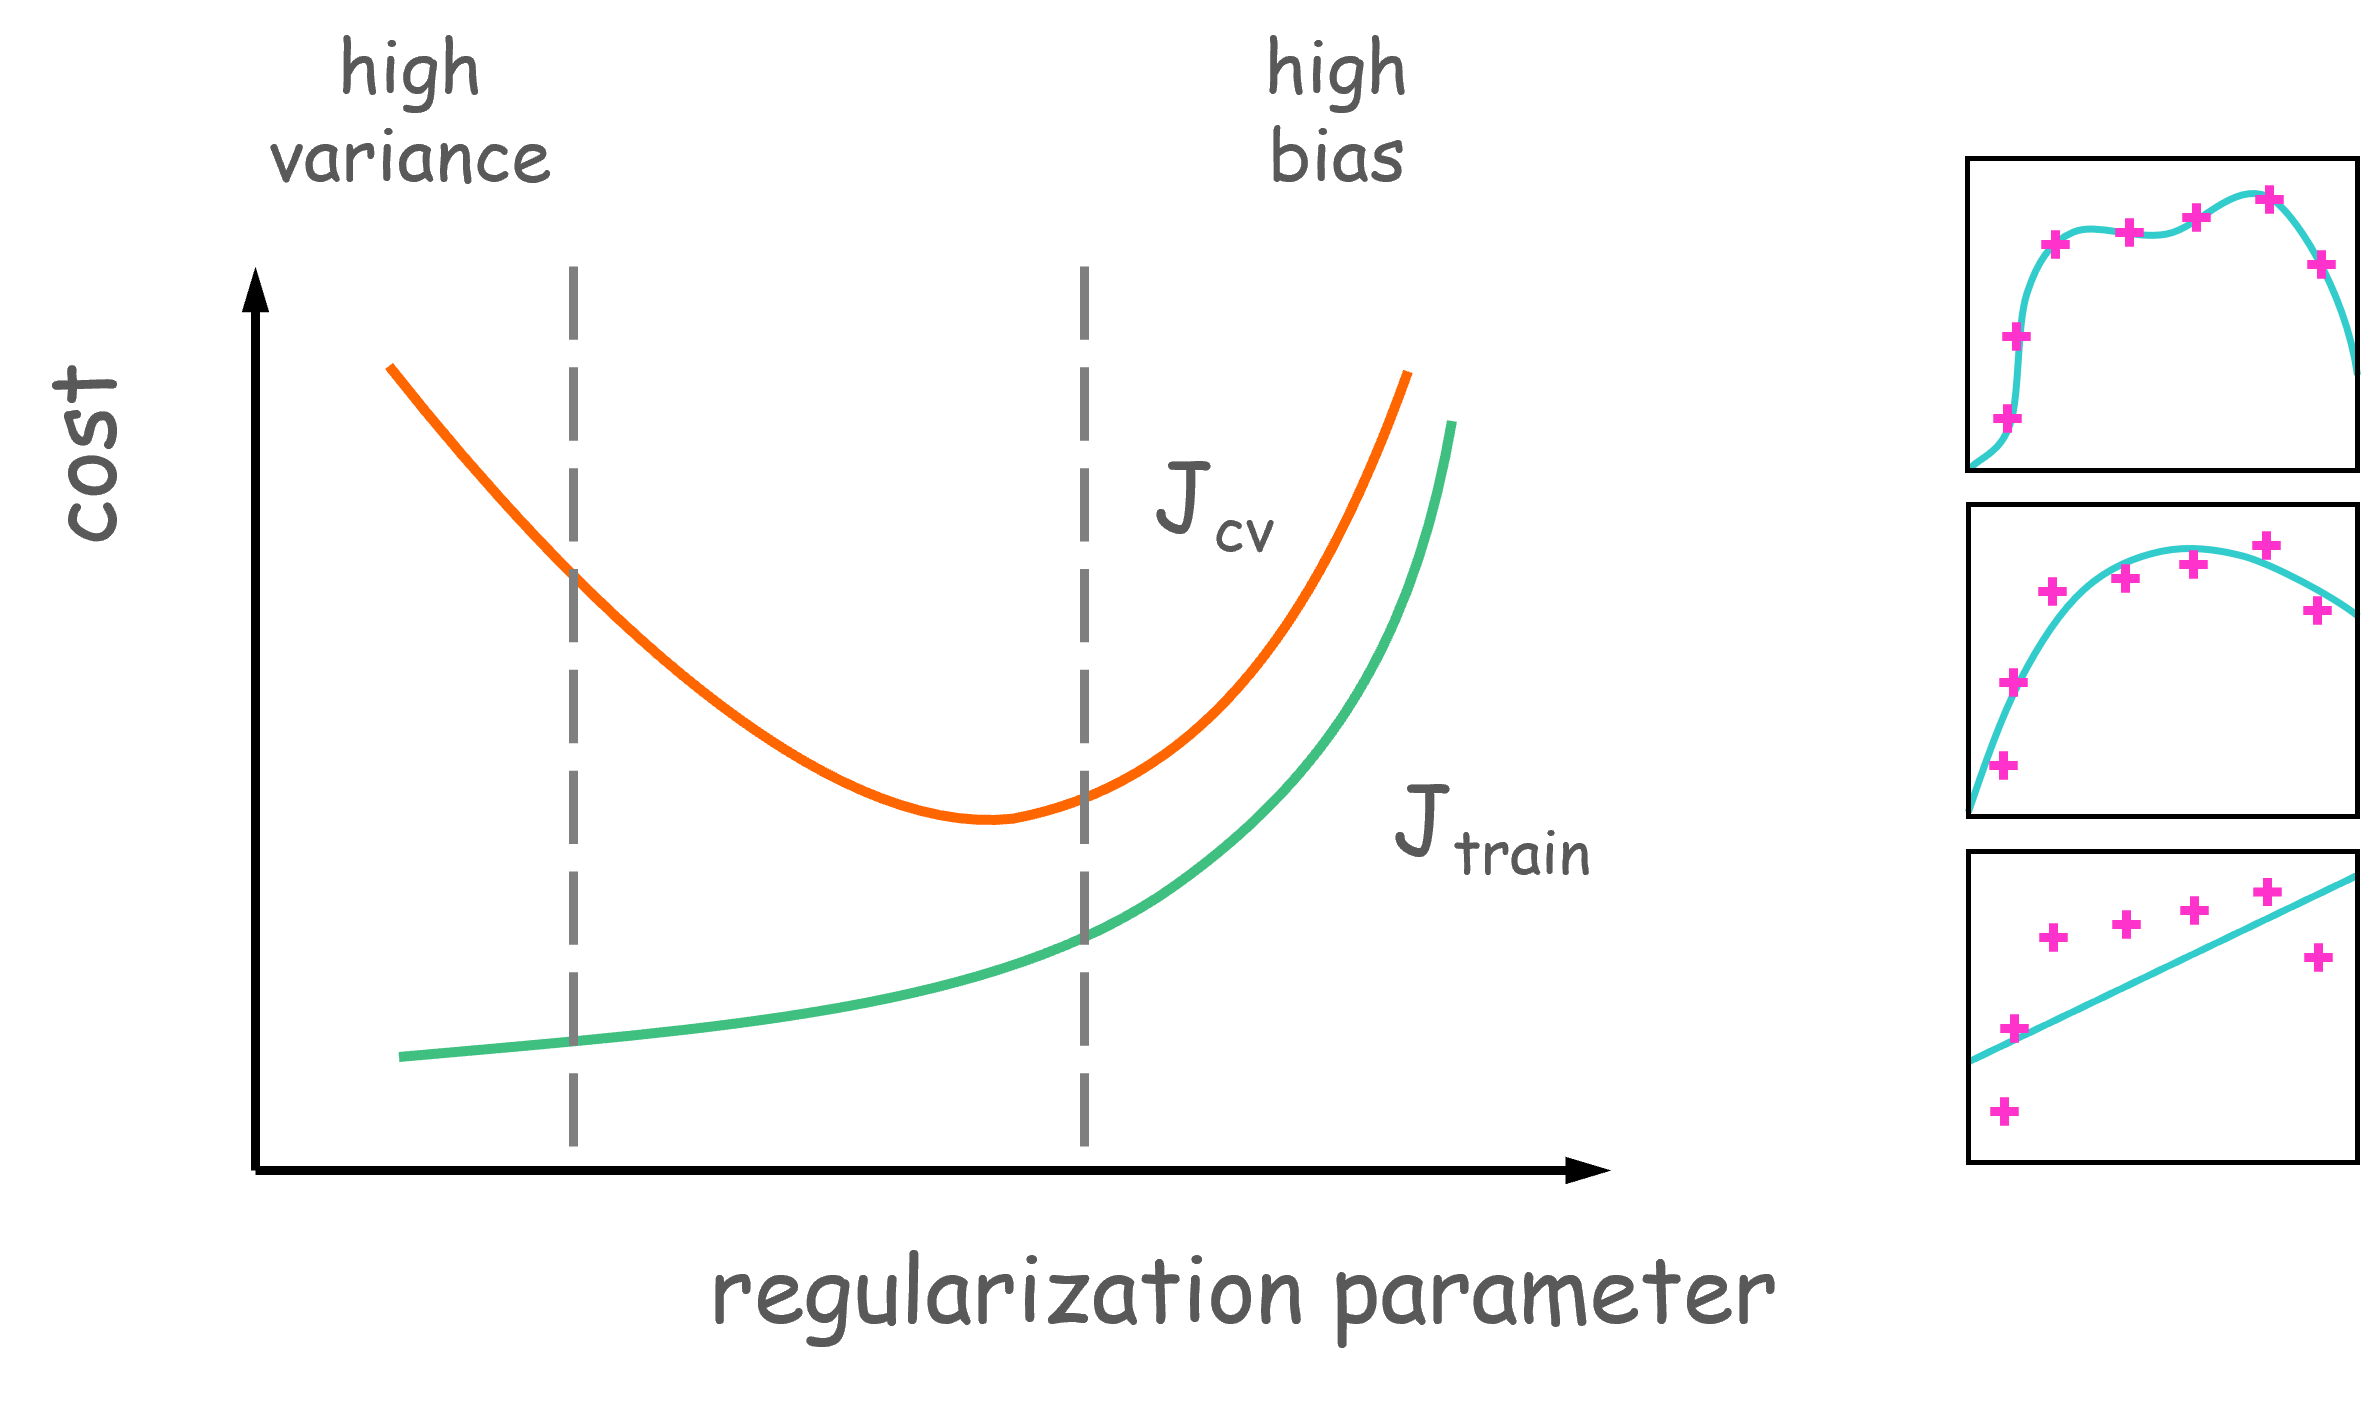
\includegraphics[width=3.8in]{./images/diagnose_regularization_parameter.png}
        \caption{Diagnose regularization parameter $\lambda$}
    \end{figure}

    \item Diagnose training set size
    \begin{figure}[H]
        \centering
        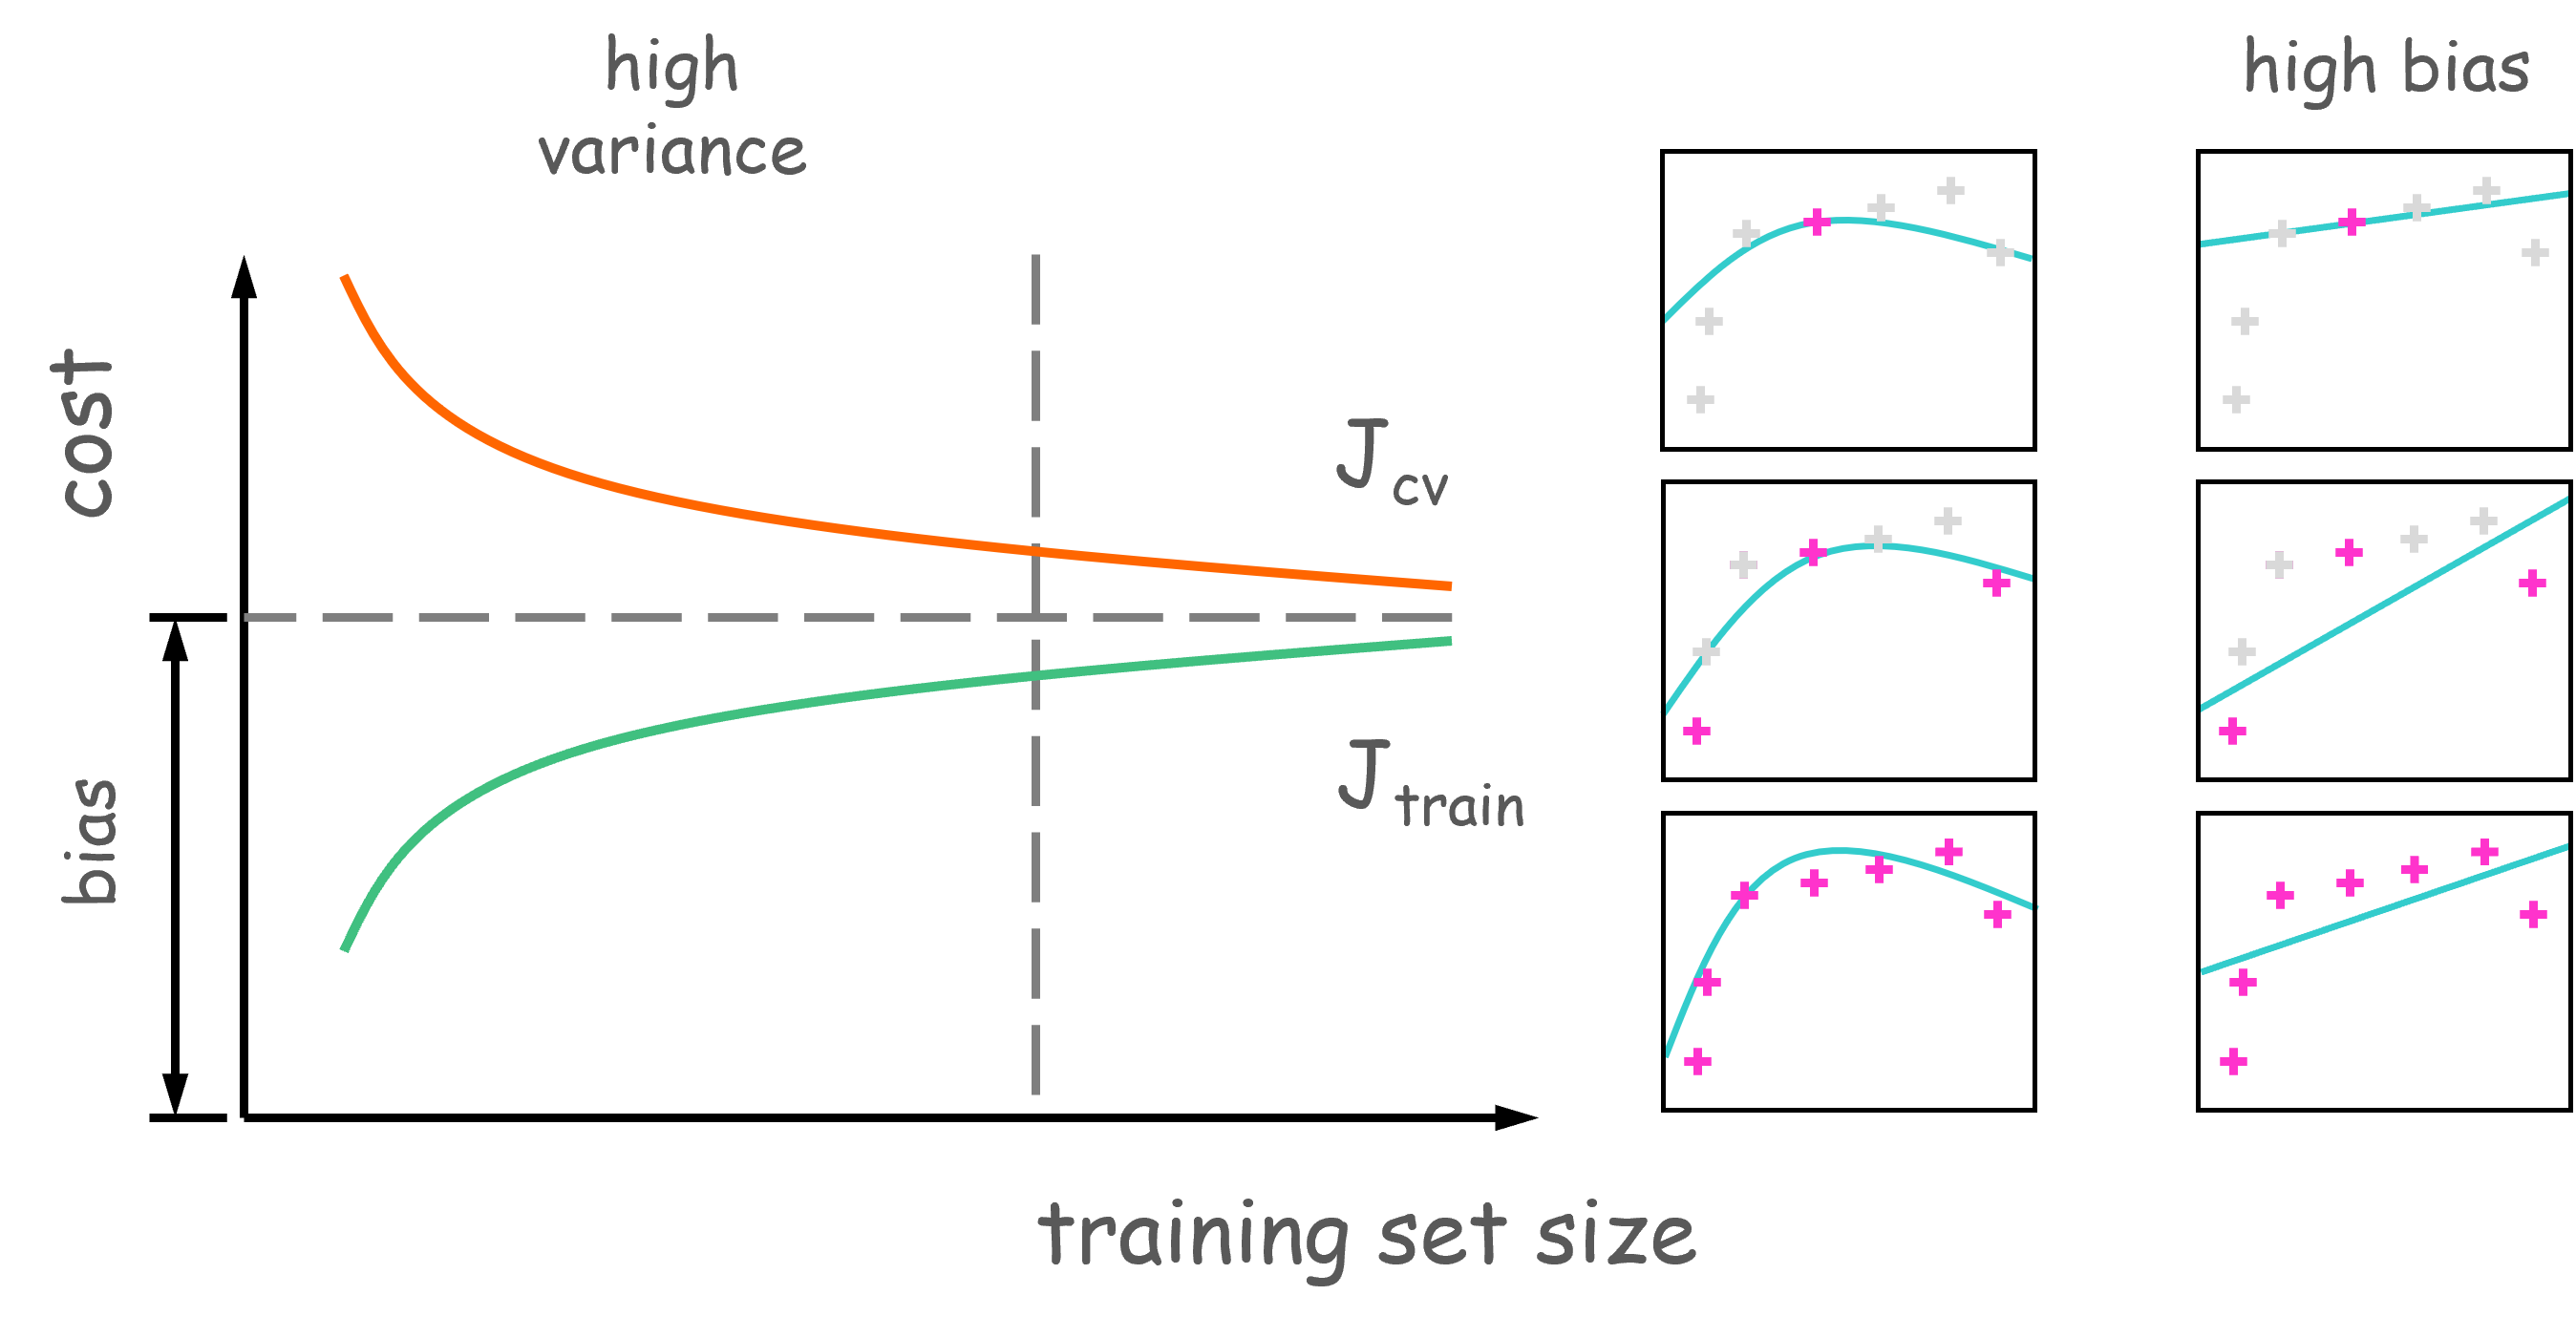
\includegraphics[width=3.8in]{./images/diagnose_training_set_size.png}
        \caption{Diagnose training set size $m$}
    \end{figure}

\end{itemize}


\section{Error analysis}
\begin{itemize}
    \item Define the error metrics
    \begin{table}[H]
        \renewcommand\arraystretch{1.5}
        \caption{Error metrics}
        \centering
        \begin{tabular}{ccc}
            \hline %%%%%%%%%%%%%%%%%%%%%%%%%%%%%%%%%%%%%%%%%
            Cases      & Actual 1       & Actual 0       \\ 
            \hline %%%%%%%%%%%%%%%%%%%%%%%%%%%%%%%%%%%%%%%%%
            Predict 1  & True positive  & False positive \\ 
            Predict 0  & False negative & True negative  \\
            \hline %%%%%%%%%%%%%%%%%%%%%%%%%%%%%%%%%%%%%%%%%
        \end{tabular}
    \end{table}

    \item Define precision $P$ and recall $R$
    \begin{equation}
        \begin{aligned}
            P &= \frac{\text{True pos.}}{\text{True pos.} + \text{False pos.}} \\
            R &= \frac{\text{True pos.}}{\text{True pos.} + \text{False neg.}} \\
        \end{aligned}
    \end{equation}
    
    We want both precision $P$ and recall $R$ could approximate 1, but there is a trade-off between these two values.
    For a higher threshold, the precision $P$ would increase but the recall $R$ would decrease
    \begin{figure}[H]
        \centering
        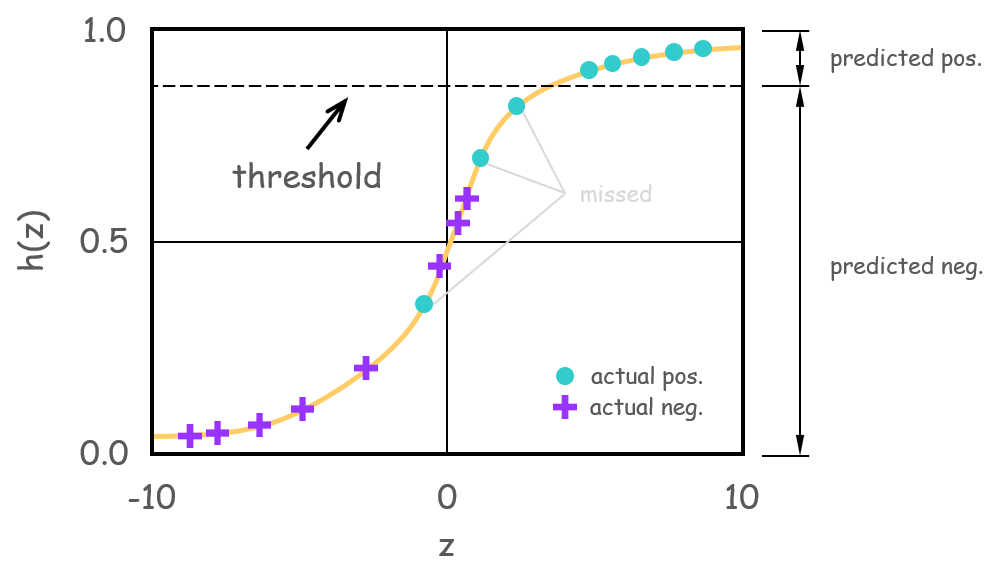
\includegraphics[width=3.8in]{./images/error_highPrecisionLowRecall.png}
        \caption{High precision low recall}
    \end{figure}
    
    \begin{table}[H]
        \renewcommand\arraystretch{1.5}
        \caption{Higher threshold}
        \centering
        \begin{tabular}{lcc}
            \hline %%%%%%%%%%%%%%%%%%%%%%%%%%%%%%%%%%%%%%%%%%%%%%%%%%%%%%%%%%%%%%%%%%%%%%%%%%%%%%%%%%%%
            Cases      & Before ($\text{threshold} = 0.5$)     & After ($\text{threshold} > 0.5$)    \\ 
            \hline %%%%%%%%%%%%%%%%%%%%%%%%%%%%%%%%%%%%%%%%%%%%%%%%%%%%%%%%%%%%%%%%%%%%%%%%%%%%%%%%%%%%
            Precision  & $\frac{7}{7+2} = 0.778$               & $\frac{5}{5+0} = 1.000$             \\ 
            Recall     & $\frac{7}{7+1} = 0.875$               & $\frac{5}{5+3} = 0.625$             \\
            \hline %%%%%%%%%%%%%%%%%%%%%%%%%%%%%%%%%%%%%%%%%%%%%%%%%%%%%%%%%%%%%%%%%%%%%%%%%%%%%%%%%%%%
        \end{tabular}
    \end{table}  
    
    For a lower threshold, the recall $R$ would increase but the precision $P$ would decrease
    \begin{figure}[H]
        \centering
        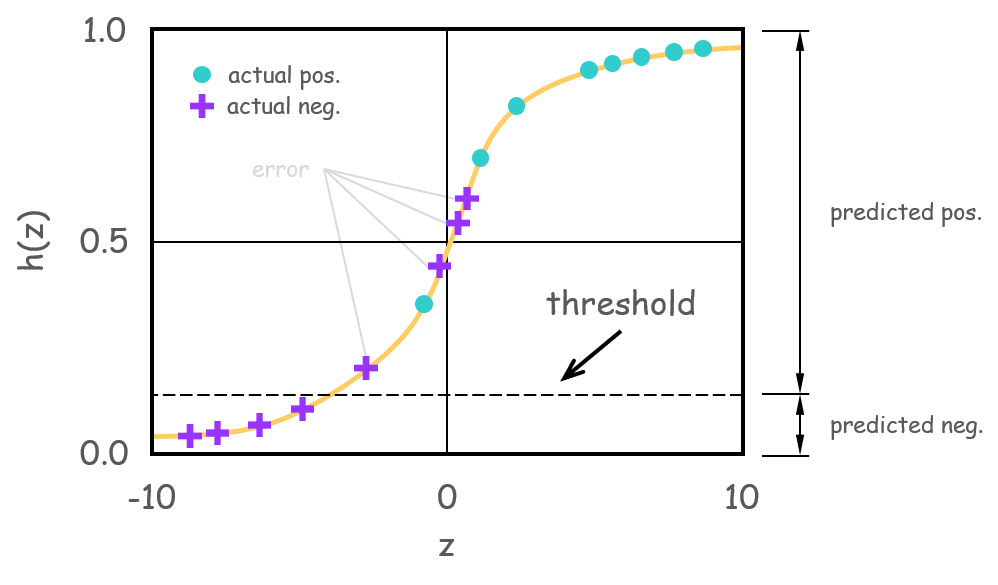
\includegraphics[width=3.8in]{./images/error_lowPrecisionHighRecall.png}
        \caption{Low precision high recall}
    \end{figure}
    
    \begin{table}[H]
        \renewcommand\arraystretch{1.5}
        \caption{Lower threshold}
        \centering
        \begin{tabular}{lcc}
            \hline %%%%%%%%%%%%%%%%%%%%%%%%%%%%%%%%%%%%%%%%%%%%%%%%%%%%%%%%%%%%%%%%%%%%%%%%%%%%%%%%%%%%
            Cases      & Before ($\text{threshold} = 0.5$)     & After ($\text{threshold} < 0.5$)    \\ 
            \hline %%%%%%%%%%%%%%%%%%%%%%%%%%%%%%%%%%%%%%%%%%%%%%%%%%%%%%%%%%%%%%%%%%%%%%%%%%%%%%%%%%%%
            Precision  & $\frac{7}{7+2} = 0.778$               & $\frac{8}{8+4} = 0.667$             \\ 
            Recall     & $\frac{7}{7+1} = 0.875$               & $\frac{8}{8+0} = 1.000$             \\
            \hline %%%%%%%%%%%%%%%%%%%%%%%%%%%%%%%%%%%%%%%%%%%%%%%%%%%%%%%%%%%%%%%%%%%%%%%%%%%%%%%%%%%%
        \end{tabular}
    \end{table}  
    
    \item The F-score or F-measure is a measure of a test's accuracy. It is calculated from the precision and recall of the test,
    \begin{equation}
        F_1 = 2 \frac{PR}{P+R}
    \end{equation}
    
    This is better than using an average equation like $\frac{P+R}{2}$.
    

\end{itemize}

 